% This is samplepaper.tex, a sample chapter demonstrating the
% LLNCS macro package for Springer Computer Science proceedings;
% Version 2.21 of 2022/01/12
%
\documentclass[runningheads]{llncs}
%
\usepackage{changepage}
\usepackage{mathtools}
\usepackage{graphicx}
\usepackage{xcolor}
\usepackage{tcolorbox}
\usepackage{makeidx}
\usepackage{float}
\usepackage{graphicx}
\usepackage{makeidx}  % allows for indexgeneration
\usepackage[english]{babel} % un troisième package
\usepackage{amssymb}
\usepackage{syntax}
\usepackage{multirow}
\usepackage{array}
%\usepackage[table]{xcolor}
\usepackage{colortbl}
\usepackage{enumitem}
\usepackage{booktabs}
\usepackage{listings}
%\usepackage{verbatim}
\usepackage{caption}
\usepackage{subcaption}
\usepackage{courier}
\usepackage{amsmath}
\usepackage{mathtools}
\usepackage{wasysym}
%\usepackage[sort=appearance]{spbasic}
%\usepackage{mathrsfs}
%\usepackage{sectsty}
%\usepackage{mathrsfs}
%\usepackage[numbers]{natbib}
%\usepackage[numbers,sort]{natbib}
%\usepackage[numbers]{natbib}
%\usepackage[backend=biber,style=numeric,sorting=none]{biblat‌ex}
%\bibliographystyle{unsrt}
%\setcitestyle{authoryear,open={(},close={)}}
%\setcitestyle{square,aysep={},yysep={;}}
%\usepackage[sort&compress]{natbib}
%\usepackage{amsthm}
%\usepackage{mathrsfs}
%\usepackage[authoryear]{natbib}
%\usepackage{amsthm}
\usepackage{tikz}
\usepackage[linesnumbered]{algorithm2e}
%\usepackage{algorithm}
%\usepackage{algorithmic}
\usepackage{algpseudocode}
\definecolor{bluekeywords}{rgb}{0.13, 0.13, 1}
\definecolor{greencomments}{rgb}{0, 0.5, 0}
\definecolor{redstrings}{rgb}{0.9, 0, 0}
\definecolor{graynumbers}{rgb}{0.5, 0.5, 0.5}
\definecolor{lightgray}{rgb}{0.83, 0.83, 0.83}
\definecolor{magnolia}{rgb}{0.93, 1.96, 1.3}


%\newtcolorbox{units}{before=\par\smallskip\centering,after=\par,hbox}

\definecolor{commentgreen}{RGB}{2,112,10}
\definecolor{eminence}{RGB}{108,48,130}
\definecolor{weborange}{RGB}{255,165,0}
\definecolor{frenchplum}{RGB}{129,20,83}
\definecolor{teagreen}{rgb}{0.82, 0.94, 0.75}
\definecolor{asparagus}{rgb}{0.53, 0.66, 0.42}
\usepackage[hyphens]{url}
\usepackage{hyperref}
\hypersetup{
  colorlinks,
  citecolor= 	blue,
  linkcolor= 	blue,
  urlcolor= 	blue}
    \usepackage{breakurl}
    \hypersetup{colorlinks=true,breaklinks=true}
  \usepackage{eucal}
  \usepackage{tabularx}
\usepackage{rotating}

\usepackage{listings}     
\usepackage{lstautogobble}  % Fix relative indenting
\usepackage{color}          % Code coloring
\usepackage{zi4}            % Nice font

\usepackage{lineno}



%\linenumbers


\DeclareCaptionFont{white}{\color{white}} 
\DeclareCaptionFormat{listing}{\colorbox{gray}{\parbox{\dimexpr\linewidth-1.9\fboxsep\relax}{#1#2#3}}}

\captionsetup[lstlisting]{format=listing,labelfont=white,textfont=white} 

\newcommand{\gtext}[1] {\textcolor{forestgreen}{#1}}


\newcommand{\keyw}[1] {\texttt{\textbf{#1}}}

\newcommand{\ie}{i.e., }
\definecolor{forestgreen}{rgb}{0.0, 0.5, 0.0}

\definecolor{aliceblue}{rgb}{0.94, 0.97, 1.0}



\newcommand{\eclipse}[1] {\textcolor{eminence}{\texttt{\textbf{#1}}}}

\newcommand{\num}[1] {\texttt{#1}}

\newcommand{\key}[1] {\texttt{\textbf{#1}}}


\newcommand{\sset}[1] {\llbracket #1 \rrbracket}

\newcommand{\eg}{e.g. }

\newcommand{\ai}{ Artificial Intelligence}

\newcommand{\ecircle}[1] {\textcircled{{\small #1}}}

\newcommand{\cmt}[1] {\textcolor{black}{#1}}


\newcommand{\tab}[1]{Table \ref{#1}}

\newcommand{\algo}[1]{Algorithm \ref{#1}}

\newcommand{\commenting}[1] {\textcolor{blue}{#1}}

\newcommand{\quot}[1] {``#1''}

\newcommand{\emath}[1] {$#1$}

\newcommand{\emathtt}[1] {$\mathtt{#1}$}

\newcommand{\msym}[1] { $\mathscr{#1}$ }

\newcommand{\alg}[1] {Algorithm \ref{#1}}

\newcommand{\lst}[1] {Listing \ref{#1}}

\newcommand{\link}[2] {\texttt{#1}$\rightarrow$ \texttt{#2}}

\newtheorem{mydef}{\normalfont \textbf{Definition}}

\newcommand{\AB}[1] {\textcolor{red}{#1}}

\newcommand{\BH}[1] {\textcolor{blue}{#1}}

\newcommand{\gl}[1] {\langle {#1} \rangle}
\newcommand{\effect} {\textrm{Effect}}
\newcommand{\push} {\textrm{Push}}
\newcommand{\pull} {\textrm{Pull}}

\newcommand\myeq{\stackrel{\mathclap{\footnotesize\mbox{def}}}{=}}

% draw a frame around given text
\newcommand{\framedtext}[1]{%
\par%
\noindent\fbox{%
    \parbox{\dimexpr\linewidth-2\fboxsep-2\fboxrule}{#1}%
}%
}

\definecolor{commentgreen}{RGB}{2,112,10}
\definecolor{eminence}{RGB}{108,48,130}
\definecolor{weborange}{RGB}{255,165,0}
\definecolor{frenchplum}{RGB}{129,20,83}

\newcommand{\code}[1] {\texttt{#1}}

%\spnewtheorem{myexample}{Example}[section]{\bfseries}{\itshape}


\usepackage{tikz}
\usetikzlibrary{calc}
\usepackage{tcolorbox}

%%%%%%%%%%%%%%%%%%%%%%%%%%%%%%%%%%%%%%
\usetikzlibrary{calc,shadows.blur}
\tcbuselibrary{skins} % Assuming you have the "skins" library installed

\newtcolorbox{resp}[2][]{%
  enhanced jigsaw,
  colback=white,%
  colframe=gray,
  size=small, % Choose which "size=small" to keep
  boxrule=1pt,
  title=#2,
  halign title=flush center,
  coltitle=black,
  drop shadow=black!3!white,
  attach boxed title to top left={xshift=1cm,yshift=-\tcboxedtitleheight/2,yshifttext=-\tcboxedtitleheight/2},
  minipage boxed title=3cm,
  boxed title style={%
    colback=white,
    size=fbox, % Choose which "size=fbox" to keep
    boxrule=1pt,
    boxsep=2pt,
    underlay={%
      \coordinate (dotA) at ($(interior.west) + (-0.5pt,0)$);
      \coordinate (dotB) at ($(interior.east) + (0.5pt,0)$);
      \begin{scope}
        \clip (interior.north west) rectangle ([xshift=3ex]interior.east);
        \filldraw [white, blur shadow={shadow opacity=60, shadow yshift=-.75ex}, rounded corners=2pt] (interior.north west) rectangle (interior.south east);
      \end{scope}
      \begin{scope}[gray!80!black]
        \fill (dotA) circle (2pt);
        \fill (dotB) circle (2pt);
      \end{scope}
    },
  },
  #1, % Move "Learned" to before the closing curly brace
}%

\newtcolorbox{boxD}{
    colback = white, 
    colframe = black, 
    boxrule = 0pt, 
    toprule = 3pt, % top rule weight
    bottomrule = 3pt % bottom rule weight
}
\newtcolorbox{boxF}{
    colback = yellow!5!white,
    enhanced,
    boxrule = 1.5pt, 
    colframe = white, % making the base for dash line
    borderline = {1.1pt}{0pt}{main, dashed} % add "dashed" for dashed line
}

\newtcolorbox{boxC}{
    colback = blue!0!white,  % background color
    boxrule = 0pt  % no borders
}
\newcommand{\fig}[1]{Figure \ref{#1}}
%%%%%%%%%%%%%%%%%%%%%%%%%%%%%%%%%
% Exercise Environment
%\newenvironment{exercise}{\exerciseinner\mbox{}\par\bigskip}{\endexerciseinner}
%\newcommand{\theexercise}{\theexerciseinner}

% Exercise Environment
%\tcolorboxenvironment{exercise}{
%  breakable,
%   enhanced,
%   colback=gray!7!white,
%   parbox=false, drop fuzzy shadow
%}

%%%%%%%%%%%%%%%%%%%%%%%%%%
\DeclareCaptionFont{white}{\color{white}}
\DeclareCaptionFormat{listing}{%
    \colorbox{black}{\parbox{\dimexpr\textwidth-2\fboxsep}{\textbf{\textcolor{white}{#1#2#3}}}}}
\captionsetup[lstlisting]{format=listing,labelfont=white,textfont=white}


\def\llbracket{[\![}
\def\rrbracket{]\!]}

\newcommand{\CO}[1] {\langle\langle #1 \rangle\rangle}



\newcommand\setItemnumber[1]{\setcounter{enumi}{\numexpr#1-1\relax}}

\newcommand{\gparrow}[1] {\lhook\joinrel\xrightarrow{#1} }

\newcommand{\project} {  \url{https://hermes-design.github.io/ieaaie24.html} }


%\newcommand{\hermes} {\textbf{H}uman-\textbf{C}entric \textbf{C}ollaborative \textbf{A}rchitectural \textbf{D}ecision-\textbf{M}aking for \textbf{S}ecure \textbf{S}ystem \textbf{D}esign}

\newcommand{\hermes} {Human-Centric Collaborative Architectural Decision-Making for Secure System Design}


\usepackage{lineno}

\usepackage{calrsfs}
\DeclareMathAlphabet{\pazocal}{OMS}{zplm}{m}{n}
\newcommand{\La}{\mathcal{L}}
\newcommand{\Lb}{\pazocal{L}}

\def\BibTeX{{\rm B\kern-.05em{\sc i\kern-.025em b}\kern-.08em
    T\kern-.1667em\lower.7ex\hbox{E}\kern-.125emX}}

    
\begin{document}
%
\title{Applying Formal Verification to Assess Galileo Search and Human Rescue Communication Services}
\author{Abdelhakim Baouya\inst{1} \and Brahim Hamid\inst{1} \and Otmane Ait Mohamed\inst{2} \and Saddek Bensalem\inst{3} }
\institute{IRIT, Université de Toulouse, CNRS, UT2, France \\
           \email{abdelhakim.baouya@irit.fr, brahim.hamid@irit.fr}
           \and
           HVG Group, ECE Department, Concordia University, Montréal, Canada\\
           \email{otmane.aitmohamed@concordia.ca}  
           \and
           VERIMAG, Université Grenoble Alpes, CNRS, Grenoble, France\\           
           \email{saddek.bensalem@univ-grenoble-alpes.fr}   
}
%
\maketitle              % typeset the header of the contribution
%
\begin{abstract}
The Galileo Search and Rescue system (SAR) is a \cmt{critical} European maritime rescue operation. It \cmt{utilizes} a network of satellites to \cmt{determine} the location of individuals in distress. \cmt{Designed to last over 12 years}, the system \cmt{has stable components} that \cmt{adhere to fundamental trustworthiness} parameters such as Reliability, Availability, and Maintainability (RAM). These parameters are \cmt{critical} for \cmt{evaluating} the overall rescue performance in situations involving \cmt{endangered individuals.} This paper presents a novel approach that utilizes Continuous-Time Markov Chains (CTMCs) and their formal specification in Continuous Stochastic Logic (CSL) to evaluate the performance of the rescue communication service. We leverage the PRISM model checker for quantitative analysis, considering degradation scenarios within the communication elements and the evolving status of the distressed person. 

%The Galileo Search and Rescue (SAR) system is a cornerstone of European maritime rescue operations. It leverages a network of satellites to pinpoint the location of individuals in distress. With a designed lifespan exceeding 12 years, the system relies on robust components with inherent dependability parameters such as Reliability, Availability, and Maintainability (RAM). These parameters are crucial for assessing the overall rescue performance in situations involving individuals in danger. This paper presents a novel approach utilizing Continuous-Time Markov Chains (CTMCs) and their formal specification in Continuous Stochastic Logic (CSL). We leverage the PRISM model checker for quantitative analysis, considering degradation scenarios within the communication elements and the evolving status of the distressed person. 

\keywords{Galileo Search and Rescue\and Reliability\and Availability\and Performance\and PRISM}
\end{abstract}
%
%
\section{Introduction}
\label{introduction}
\begin{sloppypar}

Satellite systems have become \cmt{necessary} in modern life, fulfilling \cmt{an essential} role in \cmt{various} sectors, including maritime \cite{FRAIRE2024110874} and military operations \cite{NORRIS201144}. The increasing global demand for reliable communication has driven significant innovation within the space industry \cite{economist2024}. Given the critical nature of these systems, dependability assurance is \cmt{paramount, including} the performance assessment of operational tasks, particularly those related to human \cmt{rescues,} such as search and rescue (SAR) missions \cite{galileoperformances,galileoossdd,galileoosperformancereport}.


%Formal verification \cite{Kwiatkowskaprism2011} is a powerful technique for performance and dependability assessment of critical and complex systems. It focuses on probabilistic model checking, which involves constructing and analyzing probabilistic models, typically Markov chains or Markov processes \cite{baierprinciples2008}.
\cmt{Formal verification \cite{baierprinciples2008,Kwiatkowskaprism2011}  is a powerful technique that allows for thorough system analysis to prove the properties that ensure its correct operation.} \cmt{Different} formalisms can be \cmt{used}, each \cmt{suited} for specific \cmt{applications}. \cmt{Typical} examples include Markov Decision Processes (MDPs), Continuous-Time Markov Chains (CTMCs), and Concurrent Stochastic Games (CSGs). In contrast to simulation, which relies on analyzing results from \cmt{many} random samples, formal verification provides a mathematically rigorous and exhaustive analysis of the system's behavior.


\cmt{Our work in this} paper \cmt{illustrates} how to \cmt{effectively} model communication efficiency and verify its performance using the PRISM model checker  \cite{Kwiatkowskaprism2011}. \cmt{Although} the PRISM probabilistic model checker has been widely applied to verify the correctness and effectiveness of hardware and software designs \cite{prismmodelchecker}, its application to the specific context of SAR systems has been limited. Previous research, \cmt{including studies} \cite{Hoque2015,Yu2015,Zhaoguang2013,Baouyaseaa2024}, has \cmt{primarily concentrated} on \cmt{assessing} the dependability of the satellite itself (e.g., the US GPS Satellite). \cmt{In contrast, this} work focuses on the performance of communication services \cmt{during} request-response interactions between a person in distress and the Galileo satellite system. The Galileo satellite \cmt{handles requests}, \cmt{communicates} with ground services to process it, and \cmt{dispatches} qualified personnel to \cmt{assist distressed individuals.}. This work considers \cmt{different degradation sources} as reported in the official documentation \cite{galileoperformances,galileoossdd,galileoosperformancereport}. The satellite can be in one of three states: nominal, degraded, or severely degraded. Specific anomalies, such as loss of communication with the ground station, cause each degradation status with elapsed time in such degradation. These anomalies are collected through availability monitoring as described in \cite{galileoperformances,galileoossdd,galileoosperformancereport}. The system model is specified as a Continuous-Time Markov Chain (CTMC) \cite{Kwiatkowska2007}. Assuming constant failure and repair rates for the SAR communication services, the time to failure and repair are modeled as exponentially distributed random variables. \cmt{Furthermore}, this work introduces a \cmt{new} approach by integrating human factors into the model. Unlike \cmt{earlier} models primarily focused on technological aspects, this research \cmt{integrates} human behavior as an \quot{sensor} within the system \cite{nunes2018practical}. \cmt{This analysis investigates the crucial role of human factors, such as psychological states and environmental conditions, in the timely transmission of rescue signals. It highlights the significant impact of human behavior—particularly under stress—on the effectiveness of search and rescue (SAR) operations. By conceding these dynamics, we can enhance the overall efficiency and success of SAR missions.}

\paragraph*{Outline}The remainder of this paper is structured as follows. Section~\ref{works} reviews related work. Section~\ref{preliminaries} provides a brief background on CTMCs and the PRISM language. Section~\ref{sattelitemodel} presents our proposed modeling approach for SAR systems. We then perform a quantitative analysis of the SAR services scenarios in Section~\ref{usecase}. Finally, Section~\ref{conclusion} concludes the paper and suggests directions for future research.
\end{sloppypar}

\section{Related works}
\label{works}
\begin{sloppypar}
Concurrent Stochastic Games (CSGs) \cite{Kwiatkowska2020,Kwiatkowska2021,KNPS19,KNPS22} have been implemented in various scenarios \cite{BAOUYA2024101161}, as evidenced by the literature review in the PRISM library  \cite{prismusecase}. This research leverages a variation of the stochastic game model presented in \cite{Javier2015,Javier201152} to identify optimal adaptation strategies through collaborative human maneuvers. Notably, the work in \cite{Javier201152} incorporates the human factor as a state of availability (not as a player) within the model.  In contrast, the research presented in \cite{Ray2023,RayBanerjee2023}, focuses on Multi-access Edge Computing (MEC) and proposes a service placement policy that utilizes both static (prioritized placement) and dynamic (runtime adjustments) strategies to optimize latency, resource usage, and energy consumption.


Several relevant research papers have investigated the maintenance of satellite systems \cite{Hoque2015,Yu2015, Zhaoguang2013}. In \cite{Zhaoguang2013}, the authors propose modeling a satellite system using Continuous-Time Markov Chains (CTMCs). This approach allows them to portray the impact of various factors on satellite reliability, including failures related to solar radiation and maintenance. The authors in \cite{Hoque2015}  build upon the model presented in \cite{Zhaoguang2013} by incorporating Erlang distributions instead of the exponential distributions supported by CTMCs. This change leads to more accurate results when comparing qualitative findings. Finally, authors in \cite{Yu2015} model the system using Markov Decision Processes (MDPs) to account for communication between the satellite system and ground stations. Additionally, they utilize the \emath{\pi-calculus} to model the system's semantics. Building on the findings of \cite{Zhaoguang2013}, the authors in \cite{Zhaoguang2016} model the reliability of a satellite constellation using CTMCs. \cmt{However, the impact of human interaction on maintenance costs is not addressed in any of the contributions as a game model.}
\end{sloppypar}

\section{Preliminaries}
\label{preliminaries}
\begin{sloppypar}
Probabilistic Model Checking using PRISM \cite{Kwiatkowskaprism2011} relies on constructing a formal model, typically represented using appropriate storage structures. The verification process is then performed by applying a suite of algorithms implemented within the PRISM engine \cite{engines}. For our analysis, we employ Continuous-Time Markov Chains (CTMCs) \cite{Kwiatkowska2007}, a well-established modeling technique for evaluating reliability and performance. The CTMC involves a set of states and a transition matrix \emath{\textbf{R}: S \times S \rightarrow \mathbb{R}_{\geq 0}}.  The rate specifies the delay before a transition between states s and s' takes place \emath{\textbf{R}(s,s')}, where the probability between \emath{s} and \emath{s'} take within time t is given by the value \emath{1-e^{-\textbf{R}(s,s') \times t}}. Based on research using PRISM for CTMC modeling, as outlined in \cite{prismctmc}, exponentially distributed delays are often considered suitable for modeling electronic component lifetimes and inter-arrival times. 

The PRISM model is composed of a set of modules that can synchronize. Each module is characterized by variables and commands (or transitions). The valuations of these variables represent the state of the module. The behavior of each module is described using a set of commands, each of which follows the following format:
\[
[a] \ g \ \rightarrow \ \lambda: u
\]
This indicates that if the guard condition \( g \) evaluates to true, then the update \( u \) is enabled to occur with a rate of \( \lambda \) for action \( a \). A guard is a boolean formula constructed from the module variables. The update \( u \) is an evaluation of variables expressed as a conjunction of assignments: \emath{v_{i}' = val_{i} + \ldots + v_{n}' = val_{n}} where \( v_{i} \in V \), with \( V \) being a set of local and global variables, and \( val_{i} \) are values evaluated via expressions denoted by \( \theta \) such that \( \theta: V \rightarrow \mathbb{D} \), where \( \mathbb{D} \) is the domain of the variables.

Two types of reward functions are highlighted. The action reward function assigns a real value to each state-action. This value is accumulated when the action \( a \) is selected in the state \( s \). Additionally, the state reward function, denoted as \( r_{S} : S \longrightarrow \mathbb{R} \), assigns a real value to each state \( s \). This value is accumulated when the state \( s \) is reached.

Properties are typically expressed in Continuous Stochastic Logic (CSL) \cite{kwiatkowska2002approximate}, a stochastic variant of the well-known Computational Tree Logic (CTL).  For instance, the following property expressed in natural language: \emph{Is the probability of that eventually the system failure occurring within 100 time units is less than 0.001} is expressed  as: \emath{ P_{<0.001} [ F^{\leq 100} \ fail ]}
Here, \(fail\) is the label that refers to the system failure states. 
Regarding the reward structure, the property expressed in natural language: \emph{What is the amount of reward accumulated over a specific 100 times units ?} is expressed in CSL as:
\emath{ R\{"up"\}=? [C \leq 100]}.


\end{sloppypar}


\section{The SAR/Galileo  systems}
\label{sattelitemodel}
\begin{sloppypar}

\begin{figure}[htbp]
     \centering
     		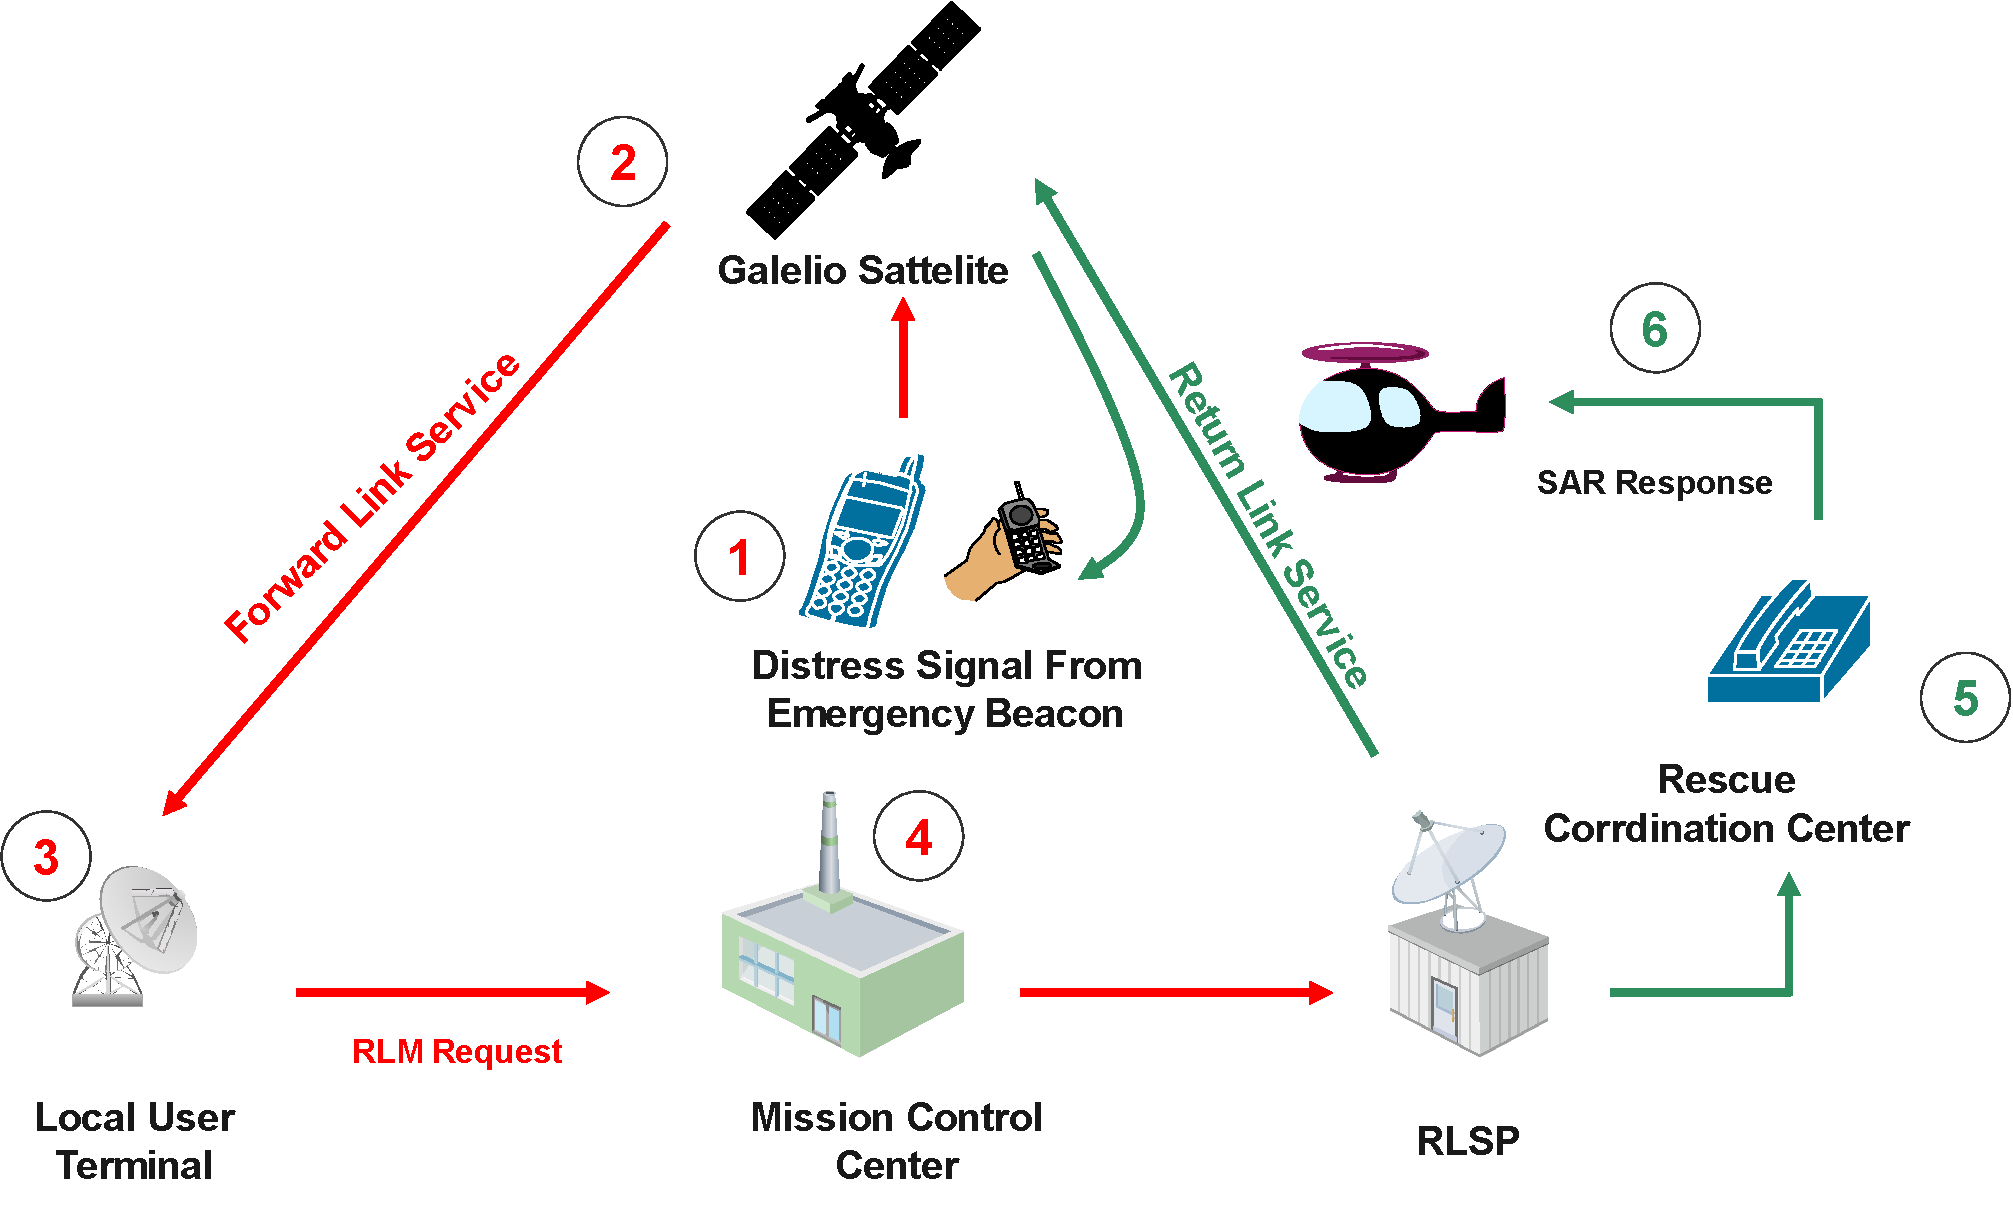
\includegraphics[width=320pt, height =200pt]{cs.pdf}
     \caption{SAR/Galileo Services \cite{galileoperformances,galileoossdd}.}
     \label{fig:usecase}
 \end{figure} 

\fig{fig:usecase} depicts the SAR/Galileo Services, illustrating the organizational structure of rescue services. The system encompasses multiple components that relay beacon signals from distressed users to rescue authorities. This section presents the system parameters and the formal response mode model.

\subsection{The system model}


COSPAS-SARSAT (C/S) is an international satellite-based Search and Rescue (SAR) distress alerting system established in 1979 by the USA, Canada, France, and the former USSR \cite{galileosarservice}.(See \fig{fig:usecase}). The full documentation is available in \cite{galileosarsdd}. The C/S system comprises:

\begin{enumerate}
    \item Beacons are 406 MHz radio transmitting devices employed in various applications. These include Emergency Position Indicating Radio Beacons (EPIRBs) and Ship Security Alert Systems (SSAS) for maritime use, Emergency Locator Transmitters (ELTs) and ELT Distress Tracking for aviation, and Personal Locator Beacons (PLBs) for individual use.

    \item The space segment \cmt{includes} satellites operating in low Earth orbit, geostationary orbit, and medium Earth orbit, responsible for processing signals transmitted by beacons.

    \item A Service Ground Segment (SGS) \cmt{consists of} a geographically distributed set of receiving ground stations known as Local User Terminals (LUTs). This network provides ground segment coverage, \cmt{allowing} the tracking of satellites and the generation of independent location estimates for user beacons.

    \item Mission Control Centers (MCC) are crucial in distributing C/S distress alerts globally and configuring the alerts for optimal response.

    \item The Sar/Galileo Ground Segment \cmt{consists of} five Reference Beacons (REFBE). These reference beacons \cmt{distibuted across} the European coverage Area are used to monitor the performance of the SAR/Galileo Service.
\end{enumerate}

The Galileo Search and Rescue (SAR) Forward link service is capable of receiving signals emitted by C/S compatible 406 MHz distress beacons (Forward Link Alert Message, as FLAM)and relaying this information to a ground segment network, known as the Local User Terminal (LUT), which consists of geographically distributed facilities deployed worldwide. The Return Link Service (RLS) enables the relay of data (Return Link Messages, or RLMs) back to the originating beacon. A primary function of the RLS is to provide the end-user of a distress beacon with automatic acknowledgment, confirming the detection of the alert and the determination of their location by the Search and Rescue (C/S) system.

Upon estimating the beacon's location, the Mission Control Center (MCC) issues an RLM\_Request. This request, covering the beacon's confirmed position, is transmitted to a backup MCC (Spanish or French). Subsequently, the RLS generates an RLM Transmission Request (RLMR) based on the original FLAM. The Galileo Core infrastructure processes the RLMR and uplinks the RLM to \cmt{appriopriate} Galileo \cmt{satellites, wich then} is broadcast to the originating beacon.

\cmt{Once the beacon receives the RLM}, sets \cmt{a} receipt status flag within FLAM. This status flag is then transmitted to the RLSP via the C/S MCC. \cmt{After} the RLSP acknowledges the receipt of the RLM, the Galileo system \cmt{stops sending} further \cmt{RLMs} to the beacon. However, if no acknowledgment of RLM reception is received within 24 hours of the initial RLM request, the Galileo system \cmt{will continue} to transmit RLMs to the beacon.

\subsection{Operational capabilities characteristics}



According to \cite{galileoperformances} and \cite{galileoossdd}, Galileo satellites \cmt{demonstrate} a reliability exceeding 88\% over a 12-year lifespan \cmt{, with} an availability of 99.5\%. \cmt{The work in} \cite{galileoosperformancereport} \cmt{reports that the availability of healthy signals from Galileo is 99.22}\%, with a recovery time of less than 15 hours. \cmt{This emphasizes the importance of ensuring timely service recovery}. Detection performance, a \cmt{crucial} aspect of the system, \cmt{refers to} the probability of successfully detecting 406 MHz beacon transmissions within the SAR/Galileo coverage area and receiving a valid beacon message at the SAR/Galileo LUT Facilities.

Three service states are defined for the SAR Forward link service in the ECA (European Coverage Area): Nominal, Degraded, and Severely Degraded. Nominal indicates normal operation. Degraded is characterized by either non-operational status for less than 24 hours continuously or less than 48 hours cumulatively over a calendar month or by losing communication with one or two ground segments (LUTs) for more than one day, or only 1 REFBE is in nominal status, or no REFBE is operational for less than 5 continuous days. Severely Degraded occurs when the SGS is non-operational for more than 24 hours continuously or more than 48 hours cumulatively over a calendar month or when communication is lost with all three LUTs and MCCs for more than four hours.

Similarly, the RLS has three service states: Nominal, Degraded, and Severely Degraded. The system is considered \quot{Degraded} if the RLSP is in degraded status or not operational for up to 7 cumulative hours within a calendar month or if RLM messages are delivered but not compliant with the latency MPL: The RLM Delivery Latency within 15 min was above or equal to 99.95\% \cite{galileoperformances}) which means that the Failure Rate is 0.05\%, and thus MTTF  is 2000 hours. \quot{Severely Degraded} status applies when the RLSP is not operational for more than 7 cumulative hours within a calendar month or if RLM messages are not delivered for more than 7 hours. In addition, based on the given availability of 99.8\% and the assumption of a very high MTBF, the estimated MTTR for the RLS would be approximately 500 hours.

\subsection{Formal modeling}

\begin{figure}[htbp]
     \centering
     		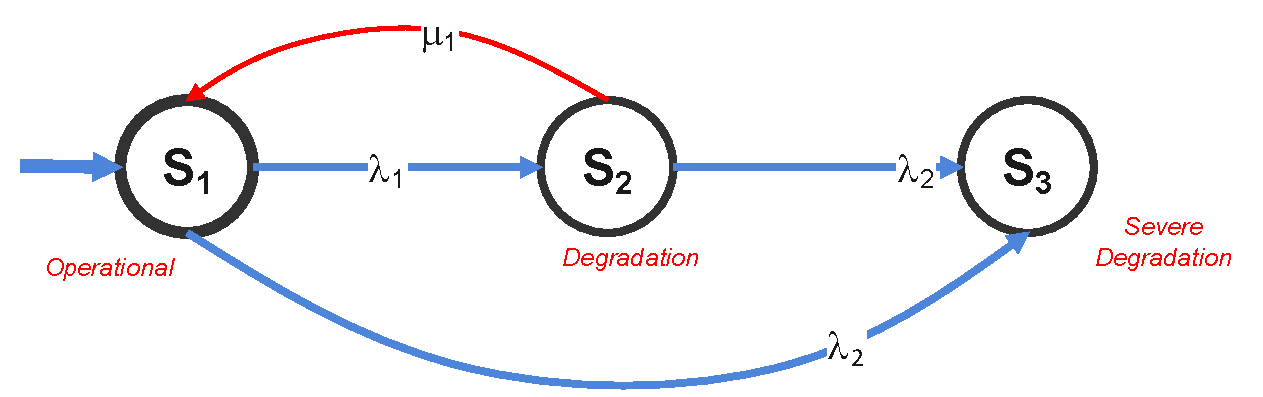
\includegraphics[width=250pt, height =80pt]{automat.pdf}
     \caption{Markov Model Pattern for SAR/Galileo Services.}
     \label{fig:model}
 \end{figure} 
 
The SAR/Galileo system can be modeled as a three-state Markov chain, illustrated in \fig{fig:model} and portrayed in the PRISM textual representation in \lst{exampleinprismtest}. State  \emath{S_{1}} represents the fully operational system, \cmt{while state} \emath{S_{2}} \cmt{indicates} a faulty state requiring recovery. State \emath{S_{3}} \cmt{signifies} a severe degradation state where maintenance is required. In the PRISM model, the system states are represented by an integer variable \emath{S}, which can take values from 0 to 3 (line 13). The assignment of degradation status relies on the constant values defined in lines 2-5. In this model, \emath{\lambda} represents the failure rate of system components, and \emath{\mu_{1}} \cmt{indicates} the recovery with repair rate. We \cmt{assume that the rates of} constant degradation and severe degradation rates (failure) follow a Poisson process. In \lst{exampleinprismtest}, the parameters are parametrizable as defined in lines 8-10. The reference documentation includes \cmt{various} sources of failure; \cmt{allowing the} model to be parametrized \cmt{so that users can} select which failures \cmt{impact} the communication system. \cmt{Additionally, this paper discusses how human reliability in sending rescue signals is} influenced by their psychological status, which we also model using a Poisson distribution. 



\lstdefinestyle{framed}
{
	frame=lrb,
	mathescape,
	numbers=left,
	belowcaptionskip=-1pt,
	xleftmargin=3.11em,
	xrightmargin=0.03cm,
	framexleftmargin=3em,
	framexrightmargin=0pt,
	framextopmargin=5pt,
	framexbottommargin=5pt,
	framesep=0pt,
	rulesep=0pt,
	numbers=left,
}

\lstset{
    breaklines=true,
    style=framed,
    escapeinside={<@}{@>},
    morekeywords={void, int, public, private, class, protected, submodules, network, connections, const, init, int, bool, double, module, rewards, endrewards, endmodule,label,ctmc},
    basicstyle=\small\ttfamily,
    keywordstyle=\bfseries\color{blue},
    morecomment=[f][\color{green!70!black}][0]{/*},
    morecomment=[l][\color{green!30!black}]{//},
    label=queueemodel
}

\begin{figure}[!htb]
\begin{minipage}{12.3cm}
\begin{lstlisting}[style=framed,
	caption=The System Status Over Execution Time,
 	label=exampleinprismtest]
ctmc    
//System states
const int Operational = 2;
const int Degraded = 1;
const int Severely_Degraded = 0;

//System performance rates
const double $\lambda_{1}$;
const double $\lambda_{2}$;
const double $\mu_{1}$;
//PRISM module
module Degradation
 S : [0..3] init Operational;
 [degradation]       S>0       $\rightarrow \lambda_{1}$:(S'=Degraded); 
 [sever_degradation] S>0       $\rightarrow \lambda_{2}$:(S'=Severely_Degraded); 
 [reset]             S=Degraded$  \rightarrow \mu_{1}$:(S'=Operational); 
endmodule

\end{lstlisting}
\end{minipage}
\end{figure}

\end{sloppypar}


\section{Quantitative analysis using PRISM}
\label{usecase}
\begin{sloppypar}
In this work, we \cmt{focus on} in evaluating signal transmission \cmt{performance using the PRISM tool}, \cmt{explicitly} focusing on scenarios where the individual experiencing distress maintains a \cmt{stable} psychological status. 

\paragraph{Experimental setup.} We have encoded properties in CSL formalism \cmt{and utilized the} PRISM model checker v4.8 \cite{Kwiatkowska2020} is utilized \cmt{for} verification. These experiments were conducted on a \cmt{system running Ubuntu with an i7 processor and equipped with 32GB RAM}. Multiple engines can be selected (refer to documentation \cite{engines}) offering performance benefits \cmt{to} specific model structures. In addition, we have implemented the scenarios outlined in \cite{Zhu2009} to accurately model attack frequencies.

\paragraph{Artifacts.} The source code for the experiments described in this section is publicly available on a GitHub repository \cite{newcas2025}. The website provides \cmt{detailed} instructions on \cmt{for replicating} the experiments.

	    \begin{resp}{\textbf{\textit{Property 1}}}
        
        \begin{equation}
        \label{eq1}\tag{\emph{\quot{Liveness}}}
         \mathtt{ P=? [ G(\quot{\textcolor{red}{up} } \xrightarrow{} \  F \ !(\quot{\textcolor{red}{up} }))  ]} 
        \end{equation}

        
        \end{resp}
        
        \normalsize

The property \ref{eq1} evaluates the signal performance by calculating the probability of the satellite successfully collecting the signal from a beacon while facing degradation of the signal, represented by the label \emath{!\quot{\textcolor{red}{up} }}. The results indicate a 100\% probability of the system transitioning from a functioning state to a degraded state. Thus, this leads us to investigate the role of degradation features on the signal transmitted through the verification of properties \ref{eq2} and \ref{eq3}.


    \begin{figure}[!htb]
    \centering
       \begin{tabularx}{\linewidth}{ m{8cm} }
           

 \begin{minipage}[t]{12cm}
     \centering

    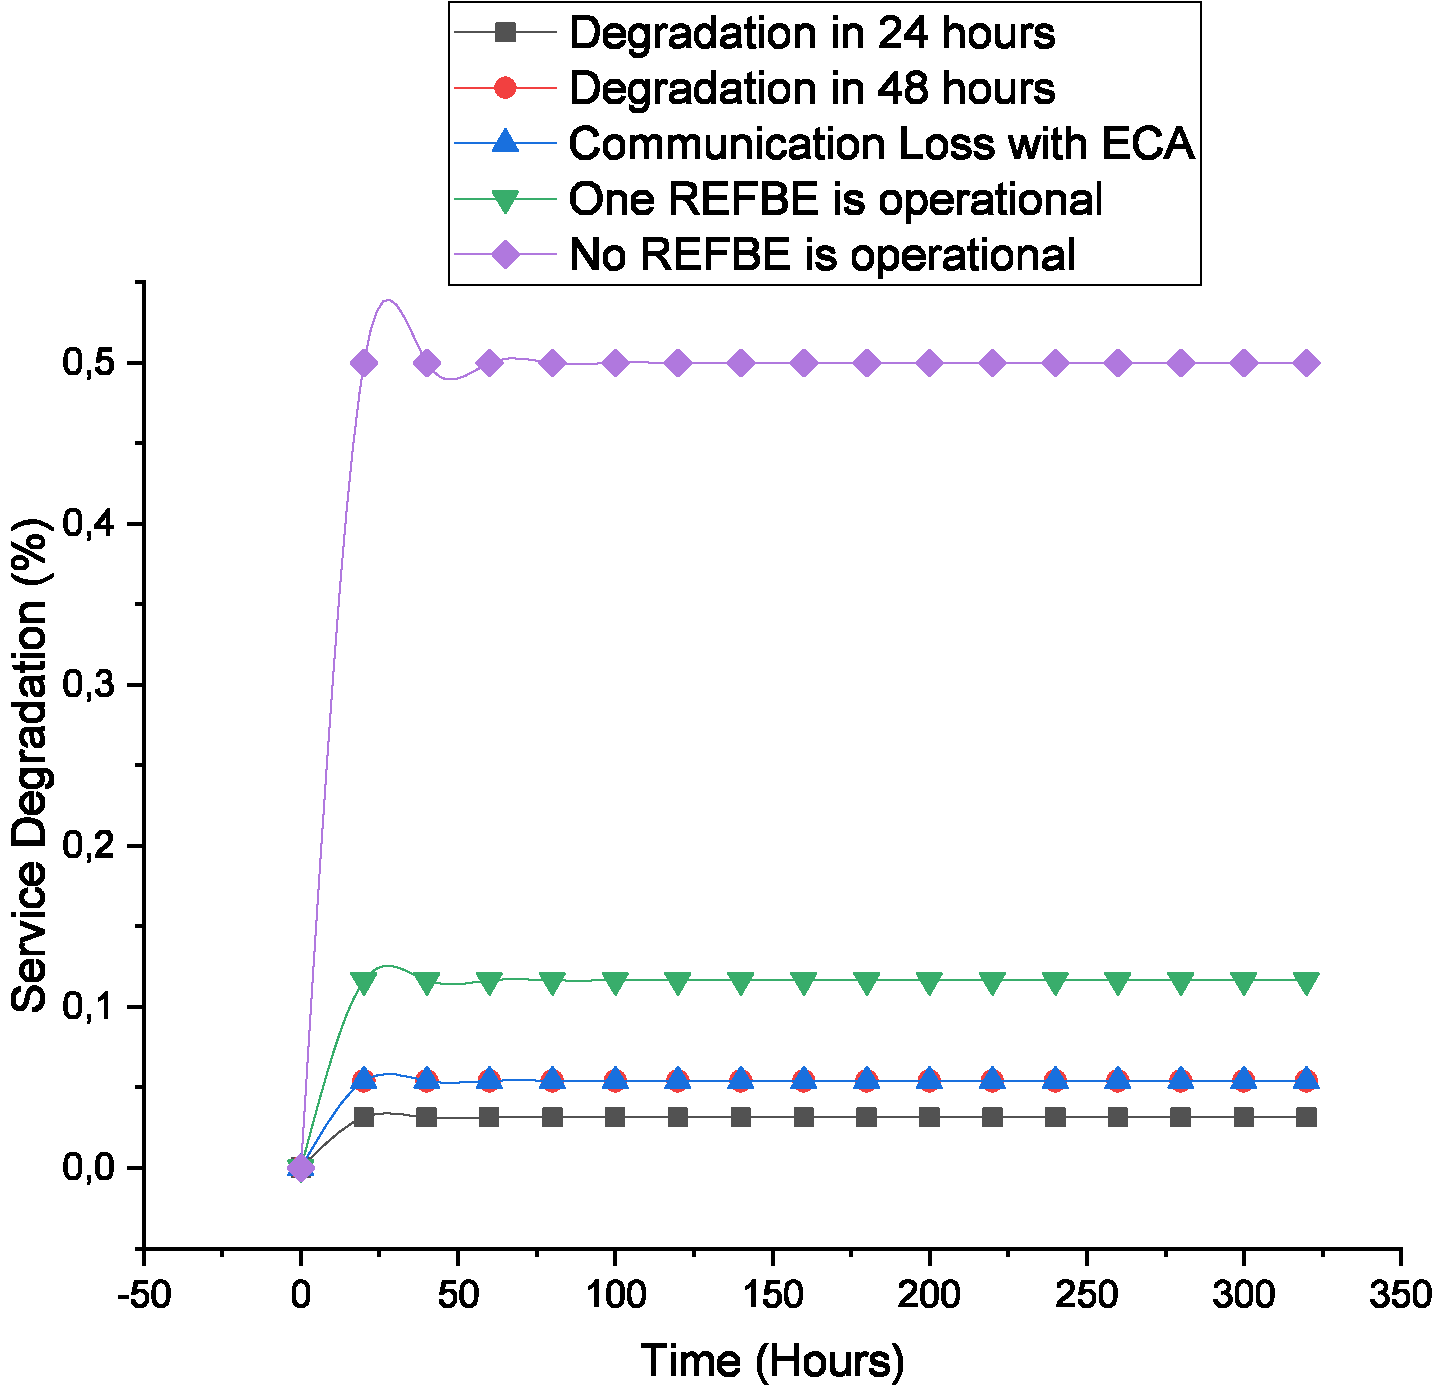
\includegraphics[width=200pt, height =180pt]{gdegraded.pdf}
    \caption{Verification of Property \ref{eq2}.}
    \label{fig:01}
   \end{minipage}
    
          \\

   \begin{minipage}[t]{12cm}
     \centering
   		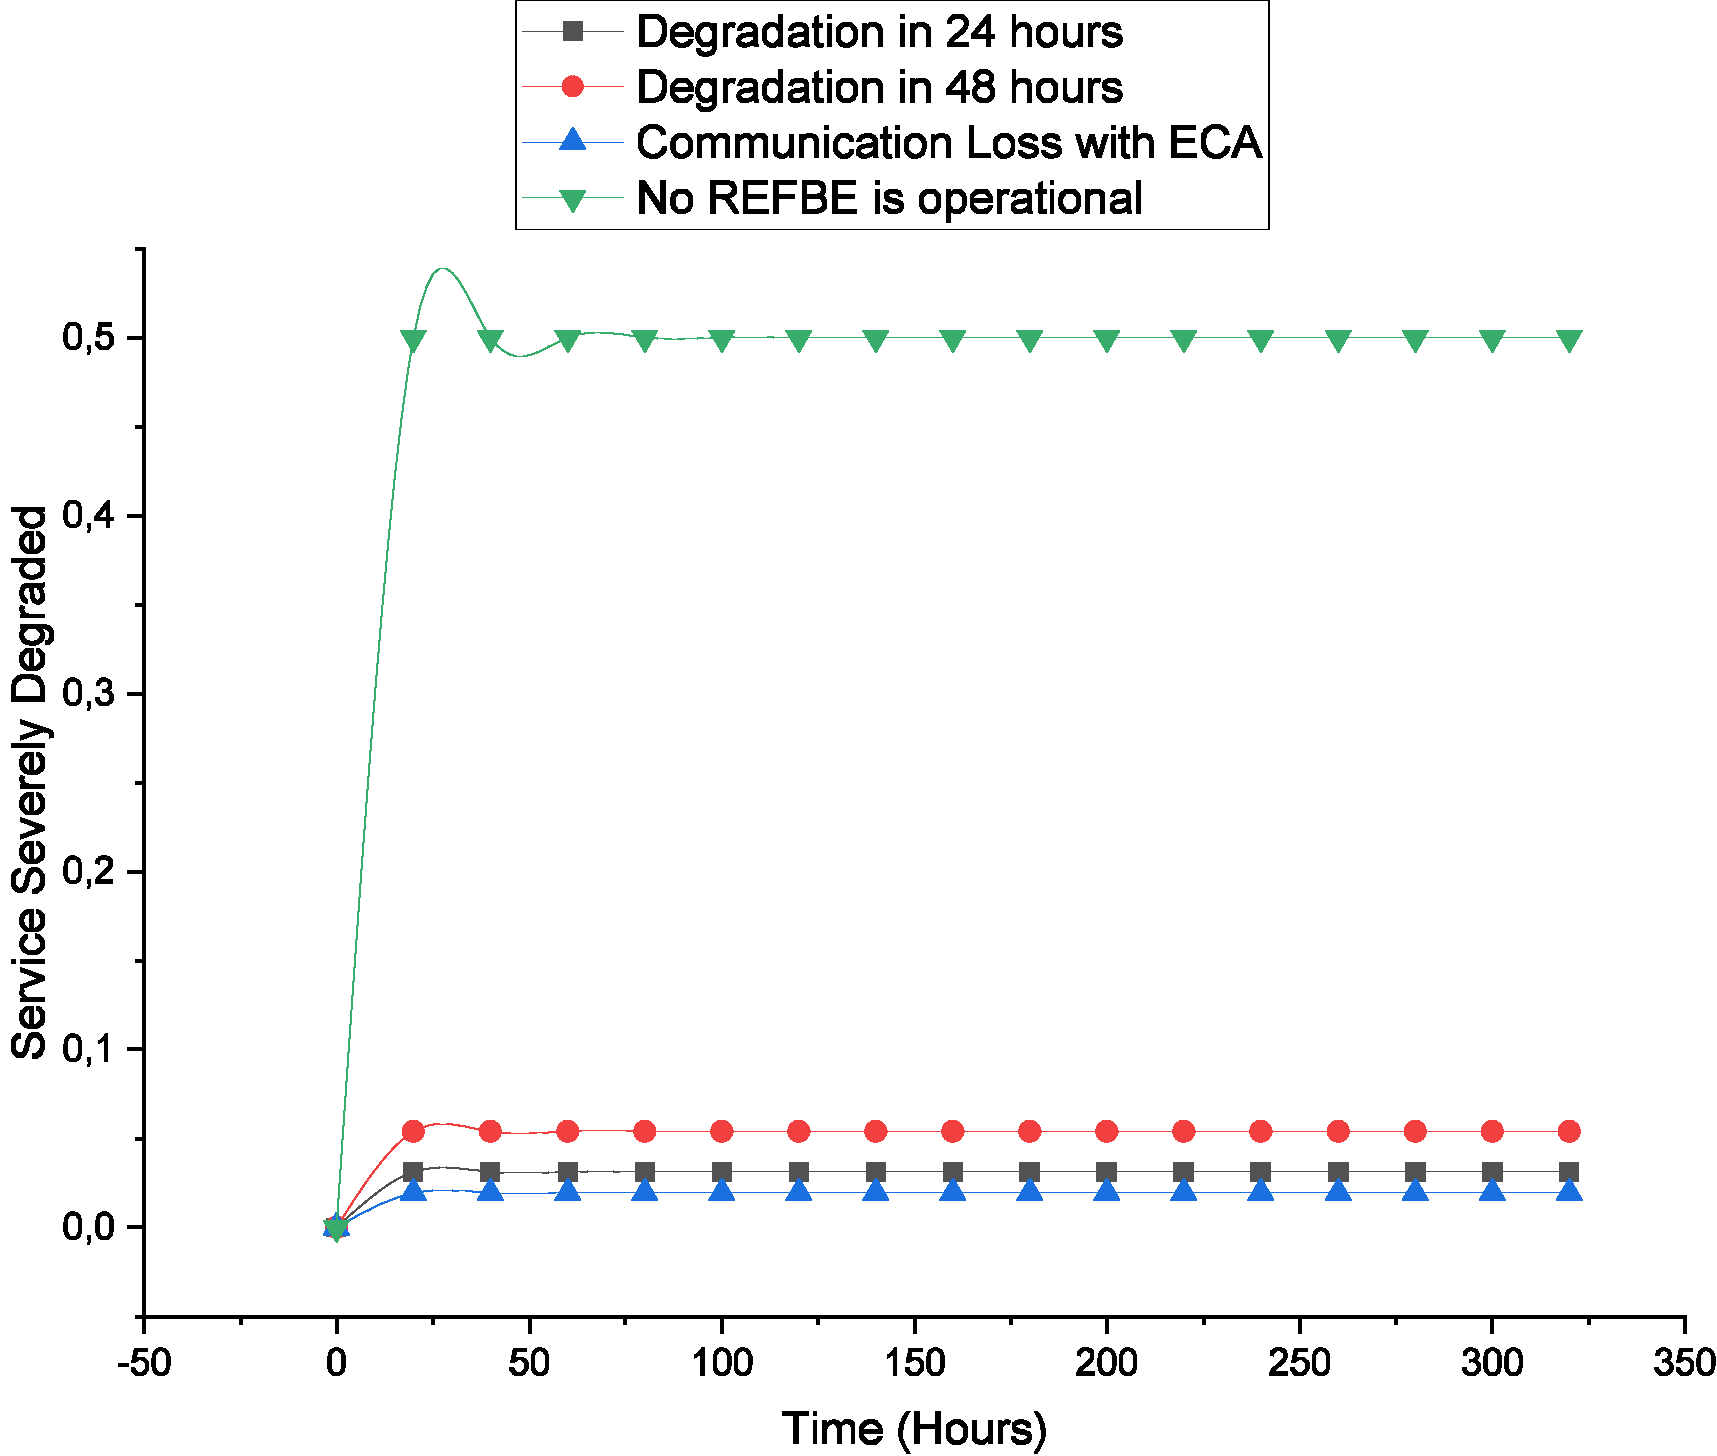
\includegraphics[width=200pt, height =180pt]{gseverlydegraded.pdf}
    \caption{Verification of Property \ref{eq3}.}
    \label{fig:02}
   \end{minipage}

               \end{tabularx}
\end{figure}


	    \begin{resp}{\textbf{\textit{Property 2}}}
        
        \begin{equation}
        \label{eq2}\tag{\emph{\quot{Degraded}}}
         \mathtt{ P=? [ (\quot{\textcolor{red}{up} }) \  U^{\leq T} \ (\quot{\textcolor{red}{Degraded} })  ]} 
        \end{equation}
        
        \end{resp}
        
        \normalsize

The property \ref{eq2} \cmt{specifies} that as time elapsed between the nominal functioning state and the degradation state increases. However, the primary distinction lies in the specific feature causing the degradation. Figure \ref{fig:01} illustrates that after 10 hours of signal transmission, the probability of degradation reaches 50\% and persists at that level for 30 calendar days due to REFBE unavailability. In contrast, internal degradation within 24 hours exhibits a low probability of 3.1\%. Notably, combining internal degradation and communication loss with ECA results in a degradation probability of 5.4\%. When only one REFBE is operational, the degradation probability reaches 11.6\%  after 20 hours of execution.


	    \begin{resp}{\textbf{\textit{Property 3}}}

        \begin{equation}
        \label{eq3}\tag{\emph{\quot{Severely Degraded}}}
         \mathtt{ P=? [ (\quot{\textcolor{red}{up} }) \  U^{\leq T} \ (\quot{\textcolor{red}{Severely\_Degraded} })  ]} 
        \end{equation}
        
        \end{resp}
        
        \normalsize


        
The property \ref{eq3} \cmt{describes} that as time elapsed between the nominal functioning state and the severe degradation state increases. However, the primary distinction lies in the specific feature causing the degradation,  \cmt{similar to the \ref{eq3} property}. Figure \ref{fig:02} illustrates that after 10 hours of signal transmission, the probability of degradation reaches 50\% and persists at that level for 30 calendar days due to REFBE unavailability. In contrast, internal degradation within 24 hours and 48 hours exhibits a low probability of 3.1\% and 5.4\%, respectively.  When communication loss with ECA, the severe degradation probability reaches 1.9\% less than the degraded mode after 20 hours of execution.

Through our analysis, we have \cmt{pinpointed} the source of service degradation within the SAR/Galileo system. \cmt{Specifically}, issues related to REFBE (Reference Beacon) monitoring of satellite performance can significantly contribute to service degradation. These \cmt{problems} can also provide maintainers with erroneous fault results, impacting maintenance activities and quality assurance.



\subsection{Discussion}
\cmt{In this study, we examined} the performance of the SAR/Galileo system, specifically focusing on degradation issues \cmt{affecting} communication between satellites and the ground stations \cmt{that assist individuals} in distress. The use case is \cmt{based on} existing documentation, and we \cmt{aim} to \cmt{evaluate} the system's \cmt{capability} to save lives by \cmt{assessing} the \cmt{communication availability of each entity involved in transmitting signals.} \cmt{Although} the signal \cmt{includes} multiple parameters not explicitly \cmt{covered} in this study, our \cmt{emphasis} remains on a high-level perspective.

The model can be extended to incorporate other factors influencing satellite signal quality, such as the impact of solar radiation, as discussed in \cite{Hoque2015,baouya2024seaa}, which can significantly affect system reliability. Furthermore, human factors should also be considered, such as an individual's \cmt{ability} to push the distress button in an \cmt{emergency promptly}. 

These results do not demonstrate the possibility that the system does not fully encompass the state of the human in terms of their reaction to danger, such as the Mean  Time To React to danger (MTTR). To address this limitation, we augment the model with a module that represents the human's status in response to a crisis in a one-month calendar. This module incorporates a formula for the rate of urgent response in line 2 of \lst{exampleinprism}: 

\begin{equation*}
\lambda_{h} = MTTR / Month 
\end{equation*}

Consequently, the model is augmented to incorporate human behavior, as illustrated in \lst{exampleinprism}. Notably, the label \quot{\textcolor{red}{\emathtt{up}}} encompasses potential human ability degradation. The PRISM command depicts a state transition from the operational mode to a degraded status for the human, upon the value of the degradation rate parameter \emath{\lambda_{h}} in line 6 of \lst{exampleinprism}. However, the correct status of the communication service depends on the system's status, which can include nominal operation, degradation, severe degradation, and the degradation of human factors in line 9.

\lstdefinestyle{framed}
{
	frame=lrb,
	mathescape,
	numbers=left,
	belowcaptionskip=-1pt,
	xleftmargin=3.11em,
	xrightmargin=0.03cm,
	framexleftmargin=3em,
	framexrightmargin=0pt,
	framextopmargin=5pt,
	framexbottommargin=5pt,
	framesep=0pt,
	rulesep=0pt,
	numbers=left,
}

\lstset{
    breaklines=true,
    style=framed,
    escapeinside={<@}{@>},
    morekeywords={void, int, public, private, class, protected, submodules, network, connections, const, init, int, bool, double, module, rewards, endrewards, endmodule,label},
    basicstyle=\small\ttfamily,
    keywordstyle=\bfseries\color{blue},
    morecomment=[f][\color{green!70!black}][0]{/*},
    morecomment=[l][\color{green!30!black}]{//},
    label=queueemodel
}

\begin{figure}[!htb]
\begin{minipage}{12cm}
\begin{lstlisting}[style=framed,
	caption=The Human Status,
 	label=exampleinprism]
const double time_to_react;
const double lambda_h=time_to_react/(30*24);

module Human_Status
 Human_Status_s : [0..3] init Operational;
 [] Human_Status_s>0 -> $\lambda_h$:(Human_Status_s'=Degraded); 
endmodule

label "up" = !degraded & !Severely_Degraded & !(Human_Status_s=Degraded);
\end{lstlisting}
\end{minipage}
\end{figure}

	    \begin{resp}{\textbf{\textit{Property 4}}}
               \begin{equation}
        \label{eq4}\tag{\quot{Rescue Service}}
         \mathtt{ P=? [ (\quot{\textcolor{red}{up} }) \  U^{\leq T} \ !(\quot{\textcolor{red}{up} })  ]} 
        \end{equation}
        \end{resp}
        
        \normalsize

        
By examining Property \ref{eq4}, which integrates human status, we observe that the system's ability to rescue a person in distress diminishes as the execution time increases, as depicted in \fig{fig:03}, regardless of the Mean Time To React (MTTR). This decrease in rescue success is attributed to the increasing likelihood of the individual experiencing a psychological state that hinders their ability to activate the distress button.

While this may seem intuitive, the verification process mathematically confirms this observation. Furthermore, the results demonstrate that the system's effectiveness depends on its capability to rescue the person in danger and crucially relies on the person's timely response to the crisis.



\begin{figure}[htbp]
     \centering
   		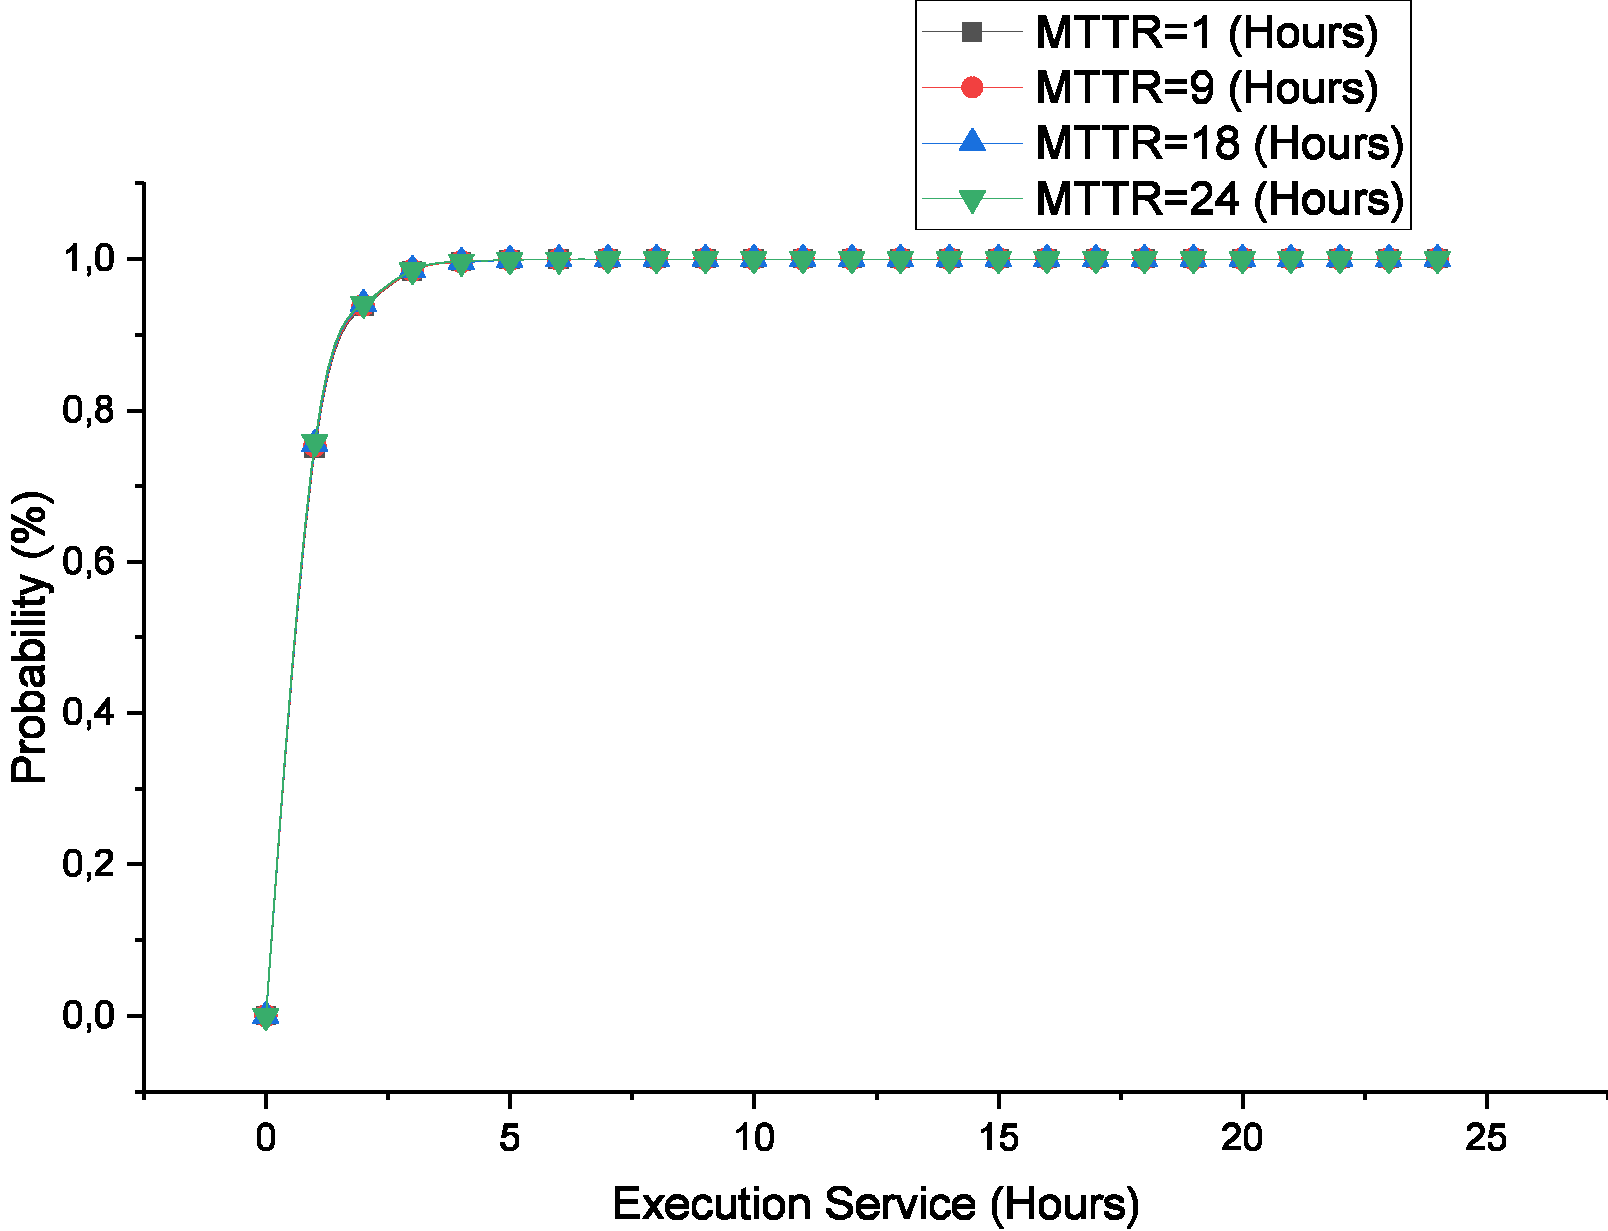
\includegraphics[width=250pt, height =180pt]{Graphh.pdf}
    \caption{Verification of Property \ref{eq4} with varied MTTR.}
    \label{fig:03}
 \end{figure} 

\subsection{Threats to validity}

This paper \cmt{focuses on specific} operational parameters of the SAR/Galileo system. \cmt{Although} other parameters \cmt{mentionned} in this SAR/Galileo documentation could \cmt{also be verified}, the PRISM model checker has limitations in supporting particular formalisms, \cmt{particulary when} incorporating satellite location and accuracy using complex data representation. These parameters necessitate high-level language specifications. \cmt{The} BIP \cite{basurigorous2011} (Behavior-Interaction-Priority) language can \cmt{effectively represent} these parameters and \cmt{facilitate} verification using a dedicated statistical model checking with SMC-BIP \cite{med2018}. 
\end{sloppypar}

\section{Conclusion}
\label{conclusion}
\begin{sloppypar}
This paper presents an approach based on CTMCs to model the communication services of the SAR/Galileo system. The captured model incorporates multiple degradation scenarios related to the observed and monitored communication between satellite systems and ground stations. We leverage the PRISM model checker for quantitative analysis, considering availability parameters and the evolving status of the distressed person.


An evaluation assessed which degradation source contributes most significantly to system failures and reduced reliability. Multiple factors were investigated, including loss of communication with monitoring ground stations and monitored failures attributed to human causes or environmental factors (the documentation does not explicitly mention the accurate sources of failures). The results demonstrate that ground stations responsible for monitoring signals are the most active sources of failures. Also, an evaluation has been performed to assess the human's capability to react to the crisis in conjunction with the system status. The results demonstrate that the \cmt{system and human parameters significantly influence performance}. 

Future work will consider incorporating additional parameters, such as the number of workstations, and exploring the implications of other formalisms, such as stochastic games, for assessing the reliability of human behavior in distress situations. The extension will also involve a comparative analysis between statistical model checkers and probabilistic model checkers to investigate the size of the resulting models and the feasibility of model verification.
\end{sloppypar}



\bibliographystyle{unsrt}
{\small
\bibliography{references}}

\end{document}
